\subsection{Objetivos}

El principal objetivo de este trabajo es analizar distinas opciones dentro de
las ofertas de plataformas para HPC (\textit{High Performance Computing}) con
el prop\'osito de presentar puntos de \textit{trade-off} entre las mismas. Con la
intenci\'on de realizar esta comparaci\'on de una manera lo m\'as realista posible,
se utilizar\'a como caso de estudio un software de din\'amica molecular (LIO) que
ha sido probado en diversas ocasiones y sobre plataformas de \textit{hardware}
muy heterogéneas. Asimismo, nuestra comparaci\'on buscar\'on ser justa en t\'erminos
de la \textit{performance} obtenida para cada una de las arquitecturas
examinadas, pero sin dejar de tener en cuenta factores tan importantes a la
hora de afrontar un desarrollo de magnitud tal como lo es portar una
aplicación ya existente: la cantidad de c\'odigo que debe ser reescrito, la
mantenibilidad del c\'odigo resultante y la disponibilidad de recursos para
asistir en el proceso.

\subsection{Arquitecturas estudiadas}

\subsubsection{Procesadores est\'andar}

Para servir de punto de comparaci\'on, en este trabajo tambi\'en analizaremos el 
comportamiento de arquitecturas como NVIDIA CUDA e Intel Xeon Phi con respecto a procesadores
CPU Estandar. En particular nos enfocaremos en la arquitectura Intel x86 de 64 bits.

Si bien las dem\'as arquitecturas analizadas difieren fuertemente de x86-64, estas diferencias
surgen de tendencias relativamente recientes en el desarrollo de procesadores que llevan a
tomar decisiones de \textit{tradeoffs} similares tambi\'en en procesadores m\'as usuales.

Una de estas tendencias es la disminuci\'on en el crecimiento de la \textit{performance} de
cada procesador o \textit{core} con respecto a a\~nos anteriores, empezando aproximadamente
desde 2003~\cite{HennessyPatterson}.

\begin{figure}[htbp]
    \centering
    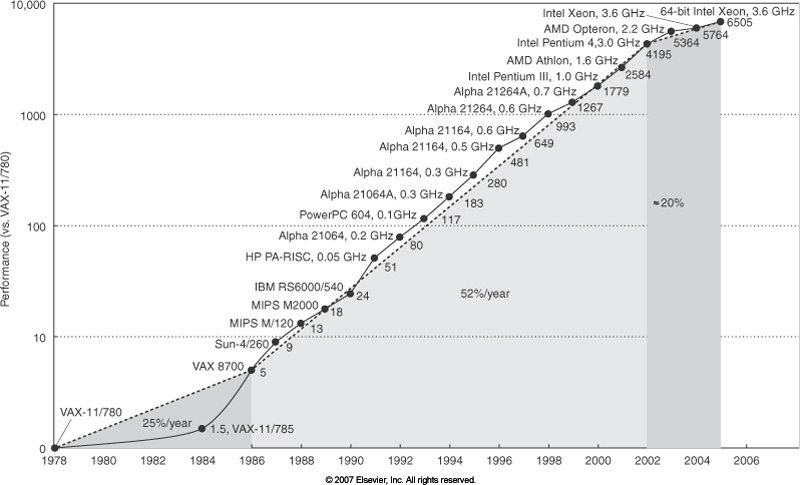
\includegraphics[width=\textwidth]{images/processor-performance.jpg}
    \caption{Performance de procesador en los \textit{benchmarks} SPEC on respecto a VAX-11/780. Tomado de~\cite{HennessyPatterson}}
    \label{processor_performance}
\end{figure}

Las razones de esto son diversas, incluyendo limites f\'isicos de cantidad de transistores
por \textit{chip} por disipaci\'on de calor, pero tambi\'en involucran otros factores 
relacionados con los tipos de \textit{paralelismo} empleados.

A grandes rasgos, existen los siguientes tipos de paralelismo que puede aprovechar una
arquitectura para mejorar la \textit{performance} de ejecuci\'on:

\begin{itemize}
    \item \textit{Instruction Level Parallelism}: Este tipo de optimizaciones, que buscan
    ejecutar la mayor cantidad de instrucciones en un mismo hilo de ejecuci\'on simultaneamente,
    eran las m\'as usuales en los monoprocesadores. Optimizaciones de este estilo incluyen
    \textit{pipelines} de procesador para ejecutar multiples instrucciones de manera solapada,
    ejecuci\'on superescalar fuera de \'orden para ejecutar multiples instrucciones que 
    utilizan unidades del procesador distintas o que no dependen una de la otra, ejecuci\'on
    especulativa (basada en predicci\'on de saltos del procesador), etc. 

    \item \textit{Data Level Parallelism}: Consideran las optimizaciones cuyo prop\'osito es
    lograr aplicar una misma operaci\'on a cada elemento de un conjunto datos simultaneamente 
    en un mismo hilo de ejecuci\'on. Concierte por ejemplo a operaciones de vectorizaci\'on, 
    presentes en procesadores de la familia Intel mediante el set de operaciones SSE 
    (Streaming SIMD Extensions) o AVX (Advanced Vector eXtensions), que incluyen instrucciones
    para actuar sobre varios enteros o valores de punto flotante (por ejemplo, sumarlos, etc.)
    que estan puestos en un arreglo, al mismo tiempo. Por eso este modelo se denomina SIMD
    (Single Instruction, Multiple Data).

    \item \textit{Thread Level Parallelism}: Alejandonos de los procesadores monocore, tenemos
    la aparici\'on de m\'aquinas con m\'as de un procesador, que permiten por lo tanto hilos
    de ejecuci\'on totalmente independientes. Estos procesadores usualmente
    comparten la memoria principal (arquitectura SMP, \textit{Symmetric Multiprocessing}), lo
    cual conlleva a esfuerzo adicional para mantener consistencia y coherencia de la misma, y
    que no se convierta en un cuello de botella.  Adem\'as, existen optimizaciones por 
    \textit{hardware} para lograr multiples hilos de ejecuci\'on en un mismo procesador
    (por ejemplo Intel Hyperthreading).
\end{itemize}

La primera de estas maneras de explotar paralelismo fue la que prevaleci\'o mucho tiempo los
procesadores dominantes en el mercado (a pesar de que la taxonom\'ia de Flynn~\cite{HennessyPatterson} ya incluye 
procesadores que explotan todas ellas). La segunda y la tercera, base de arquitecturas como NVIDIA CUDA y Xeon Phi, 
est\'an tambi\'en haciendo aparici\'on en procesadores basados en x86: El procesador Intel Xeon E7-8800 posee 10 \textit{cores}
(2 hilos de ejecuci\'on por \textit{core}) a 2.4 GHz con un set de instrucciones SSE 4.2 que permite ejecutar una misma instrucci\'on
sobre 4 valores de punto flotante IEEE-754 de 32 bits (usando registros SSE de 128 bits)~\cite{XeonE78800Spec}. 

Estas tendencias en la busqueda de lograr m\'as hilos de ejecuci\'on y m\'as procesamiento simult\'aneo de datos, adem\'as
de mejoras al nivel instrucci\'on, tiene un impacto fuerte que diferencia sistemas pensados para computo intensivo de
sistemas de prop\'osito general. Este cambio de modelo requiere m\'as esfuerzo por parte del programador para aprovecharlo
correctamente, lo cual tambi\'en genera inter\'es en herramientas y literatura que sirva de gu\'ia al desarrollador, que
ahora no puede simplemente esperar a que la performance de un procesador se duplique cada 18 meses, y debe estructurar su
c\'odigo para hacer uso de los nuevos recursos que dispone.


\subsubsection{NVIDIA CUDA}

La siguiente arquitectura analizada en este trabajo es la arquitectura GPGPU desarrollada por NVIDIA, conocida
como CUDA por las siglas en ingles de \textit{Compute Unified Device Architecture}.
CUDA surge naturalmente de la aplicaci\'on de los pipelines desarrollados para
gr\'aficos, pero aplicados a computo cient\'ifico.

Las placas de video aparecen en 1978 con la introducci\'on de Intel del iSBX 275, permitiendo dibujar lineas,
arcos y bitmaps y comunicada por DMA al procesador principal. En 1985, la Commodore Amiga incluia un coprocesador
gr\'afico que podria ejecutar instrucciones independientemente del CPU, un paso importante en la separaci\'on
y especializaci\'on de las tareas. En la decada del 90, m\'ultiples
avances surgieron en la aceleraci\'on 2D para dibujar las interfaces gr\'aficas de los sistemas operativos,
y para mediados de la d\'ecada, muchos fabricantes estaban incursionando en las aceleradoras 3D como
add-ons a las placas gr\'aficas tradicionales 2D. A principios de la d\'ecada del 2000, se agregaron los
\textit{shaders} a las placas, peque\~nos programas independientes que corrian nativo en el GPU,
y se podian encadenar entre si, uno por pixel en la pantalla.~\cite{CG} Este paralelismo es el desarrollo fundamental
que llevaba a las GPU a poder procesar operaciones gr\'aficas ordenes de magnitud m\'as rapidas que el CPU.

En el 2006, NVIDIA introduce la arquitectura G80,
que es la primera placa de video que deja de resolver \'unicamente problemas especializados a gr\'aficos
para pasar a un motor gen\'erico donde cuenta con un set de instrucciones consistente para todos los
tipos de operaciones que realiza (geometria, vertex y pixel shaders) ~\cite{cudaHandbook}. Como subproducto de esto,
el GPU deja de tener pipelines especializados y pasa a tener procesadores sim\'etricos m\'as sencillos y m\'as
faciles de construir. Esta arquitectura es la que se ha mantenido y mejorado en el tiempo, permitiendo
a las GPU escalar masivamente en procesadores simples, de un bajo clock de una disipaci\'on t\'ermica
manejable.

Los puntos fuertes de las GPGPU modernas consisten en poder atacar los problemas de paralelismo
de manera pseudo-explicita, y con esto poder escalar ``facilmente'' si solamente se corre en una
placa mas r\'apida. ~\cite{} Te\'cnicamente esta arquitectura cuenta cientos a miles de procesadores
especializados en c\'alculo de punto flotante, procesando cada uno un \textit{thread} distinto pero
trabajando de manera sincr\'onica agrupados en bloques. Cada procesador a su vez cuenta con entre
64 a 256 registros ~\cite{NvidiaFermi}~\cite{NvidiaKepler}, como porci\'on de un register file de 64kb.
Las placas cuentas con m\'ultiples niveles de cach\'e y memorias especializadas (subproducto de
su dise\~no fundamental para gr\'aficos). Estos no poseen instrucciones SIMD, ya que su dise\~no primario
esta basado en cambio, en SIMT (\textit{Single Instruction Multiple Thread}), las cuales se ejecutan en los
bloques sincronicos de procesadores. De este modo, las placas modernas como la K40 alcanzan
poder de computo de 4.3 TFLOPs de precision simple, 1.7 TFLOPs de precision doble y 288GB/sec de
transferencia, usando 2880 CUDA Cores ~\cite{NvidiaKeplerDatasheet}. Para poner en escala la concentraci\'on
de poder de calculo, estas prestaciones harian de una computadora usando solo dos de estas placas
la supercomputadora m\'as potente del mundo en Noviembre 2001 ~\cite{Top500November2001}.

Para poder correr programas explotando la arquitectura CUDA, se deben escribir de manera que
el problema se particione usando el modelo de grilla de bloques de threads. Esto implica una
reescritura completa de los c\'odigos actuales en CPU y un cambio de paradigma importante, al
dejar de tener vectorizaci\'on, paralelizaci\'on automatica y otras t\'ecnicas tradicionales
de optimizaci\'on en CPU. Sin embargo, este trabajo ha rendido sus frutos en muchos casos:
en los \'ultimos 6 a\~nos, la literatura de HPC con aplicaciones en GPU ha explotado con
desarrollos nuevos basados en la aceleraci\'on de algoritmos num\'ericos (su principal uso).
% ~\cite{meter refs a gpu montecarlos}
Adem\'as, no todas las aplicaciones deben reescribirse de manera completa. Con la introducci\'on
de las librerias CuBLAS y CuFFT, se han buscado reemplazar con minimos cambios las historicas
librerias BLAS y FFTw, piedras fundamentales del computo HPC. ~\cite{cublas} ~\cite{cufft}.

Nuevas soluciones para la portabilidad se siguen desarrollando: las librerias como Thrust ~\cite{thrust},
OpenMP4.0 ~\cite{OpenMPspec} y OpenACC 2.0 ~\cite{OpenACCSpec} son herramientas que buscan hacer el
c\'odigo agnostico al acelerador de computo que usen. Estas permiten definir las operaciones de
manera gen\'erica y dejan el trabajo pesado al compilador para que subdivida el problema de la manera
que el acelerador (CPU, GPU, MIC) necesite. Obviamente, los ajustes finos siempre quedan pendiente para
el programador especializado, pero estas herramientas representan un avance fundamental al uso
m\'asivo de t\'ecnicas de paralelizaci\'on autom\'aticas, necesarias hoy dia y potencialmente
imprescindibles en el futuro.

La aplicaci\'on LIO ya contaba con una implementacio\'n CUDA desarrollada anteriormente a este
trabajo ~\cite{TesisNitsche}. En este trab\'ajo nos encargaremos de analizar algunos detalles internos de
la arquitectura CUDA usando esa implementaci\'on de referencia, y estudiar el impacto de las distintas
mejoras considerando los progresos que han surgido en las iteraciones de CUDA desde entonces.



\subsubsection{Intel Xeon Phi}

TODO: PONER REFERENCIAS!!

La última de las arquitecturas examinadas en este trabajo es un desarrollo relativamente reciente
por parte de Intel, el coprocesador Xeon Phi. A pesar de haber ingresado en la escena de HPC hace 
menos de 3 años, se ha visto una apuesta muy fuerte a esta tecnología, como puede verse en el papel 
que juega dentro de supercomputadoras como la Tianhe-2 de la Universidad de Sun Yat-Sen en China,
listada en TOP 500 como la supercomputadora más rápida del mundo en Junio 2013, Noviembre 2013 y
Junio 2014. Esta supercomputadora de 16000 nodos, cada uno de los cuales consiste de dos Intel 
Ivy Bridge Xeon en combinación con 3 coprocesadores Xeon Phi, es teóricamente capaz de alcanzar los
54.9 petaflops de computo, y superó por casi el doble de Teraflps a su competidor más cercano en
Junio de 2013.

Esta apuesta no solo es virtud de las características técnicas del coprocesador, que promete una
capacidad de computo de 1000 GFLOPs y 240 GB/s de transferencia, sino que además ha de considerarse
que, a diferencia de su competidor directo NVIDIA CUDA y OpenCL, el esfuerzo de portar la aplicación a utilizar
el Xeon Phi es presentado como mucho menor por parte de Intel. Esta combinación de performance y portabilidad
presenta al Xeon Phi como una alternativa muy interesante en el campo de aplicaciones intensivas en cómputo.

Para lograr esto, Intel apostó al uso de una nueva arquitectura de muchos procesadores (Many Integrated Core Architecture, MIC) de
tipo SMP (Symmetric MultiProcessing), bajo el nombre en código \textit{Knights Corner}. El coprocesador dispone de 60 cores basados 
en el procesador Intel Pentium, con una ISA (Instruction Set Architecture) muy similar al set de instrucciones IA 32. Además de su cantidad 
numérica, estos cores disponen de registros SIMD (Single Instruction Multiple Data) de 512 bits (el doble de tamaño que los registros de 256
bits que disponen los procesadores de Intel basados en el set de instrucciones AVX, como el Xeon). Esto implica que programas
que ya explotan fuertemente el paralelismo a nivel datos y a nivel \textit{threads} de computo debieran poder hacer uso de 
estas impresionantes facilidades con una recompilación. Adicionalmente el coprocesador puede usarse para que el
\textit{host} delege calculos intensivos en el coprocesador (con el cual esta conectado por un bus
PCI Express de alta velocidad) y luego obtenga los resultados del mismo. Ambos modos son soportados por el \textit{toolchain} que provee
Intel, que consiste no solo de compiladores de C, C++ y Fortran, sino que también de librerías especialmente optimizadas para uso del Xeon Phi 
como lo es la Intel MKL (Math Kernel Library). 

Sin embargo, factores diversos hacen que si bien el esfuerzo de portar una aplicación ya existente para aprovechar el Xeon Phi es menor en principio
a otras opciones como NVIDIA CUDA, el mismo no es insignificante. La cantidad de cores se ve compensada por su relativa baja velocidad de clock 
(aproximadamente 1.0 GHz), lo cual requiere mas esfuerzo por parte del programador para hacer buen uso de la escalabilidad tanto en cores como en 
paralelismo en uso de los datos (vectorización), entre otros aspectos. 

Los detalles particulares de esta arquitectura y su impacto serán descriptos y analizados en capítulos posteriores. 
A pesar de su juventud, esta plataforma ha inspirado trabajos relacionados como por ejemplo [TODO: PONER CITAS DE MATERIAL SOBRE XEON PHI]. Estos trabajos
buscan dar números finos en benchmarks con el propósito de guiar al programador en su afán de explotar la performance del coprocesador. En este trabajo buscamos
poner estos pasos en contexto de otras opciones, y considerar otros aspectos relevantes al trabajo de portar \textit{software} de computo científico.


\subsection{Problema abordado}

Con la aparici\'on de las computadoras en el \'ambito de la ciencias experimentales, han
ganado tracci\'on los desarrollos en m\'etodos de simulaci\'on de modelos matem\'aticos. 
Con el apoyo de estas nuevas t\'ecnicas se hace posible no solo
complementar la experimentaci\'on sino tambi\'en explorar la teor\'ia de fondo de maneras que
no son posibles o convenientes mediante enfoques m\'as cl\'asicos.

Un ejemplo es el estudio, dentro del marco de la qu\'imica, de los comportamientos de las 
part\'iculas peque\~nas (electrones, protones, etc.) de acuerdo a las leyes de la f\'isica. En este \'area las
simulaciones de los postulados que rigen la mec\'anica de part\'iculas (denominada mec\'anica cu\'antica)
resultan invaluables para el estudio de fen\'omenos a escala microsc\'opica.

La mec\'anica cu\'antica establece que todas las propiedades de un sistema de part\'iculas peque\~nas
pueden ser obtenidas a partir de la funci\'on de onda $\Psi$ del mismo, la cual obedece la 
ecuaci\'on de onda de Schr\"odinger \textit{dependiente del tiempo},

\begin{equation}
    \label{schro_time_dep}
    -\hbar\frac{\partial \Psi}{\partial t} (\mathbf{r},t) = \frac{-\hbar^2}{2\mu}\nabla^2 \Psi(\mathbf{r},t) + V(\mathbf{r},t) \Psi(\mathbf{r},t)
\end{equation}

donde $\mathbf{r} = (r_1,\dots,r_n)$ es el vector de todas las posiciones de las part\'iculas del sistema,
$m$ es la masa de una part\'icula cualquiera, $V$ es un campo externo que afecta a las part\'iculas y
$\hbar$ es la constante de Planck divida por $2\pi$. En esta versi\'on, el campo $V$ depende del tiempo; si
esto no ocurre se puede simplificar utilizando el operador Hamiltoniano

\begin{equation*}
    \hat{H} =  -\frac{\hbar^2}{m} \nabla^2 + \hat{V}
\end{equation*}

a la ecuaci\'on de Sch\"odinger \textit{independiente del tiempo}

\begin{equation}
    \label{schro_time_indep}
    \hat{H} \Psi(\mathbf{r}) = E \Psi(\mathbf{r})
\end{equation}

Donde $E$ es la energ\'ia asociada a la funci\'on de onda $\Psi$.

Ahora, si bien resolver esta ecuaci\'on diferencial ser\'ia suficiente para determinar todas las propiedades del sistema, esto no puede hacerse de 
manera exacta cuando hay m\'as de una part\'icula en el mismo. Por este motivo, para problemas de mayor tama\~no se utilizan aproximaciones num\'ericas
para obtener una soluci\'on de~\ref{schro_time_indep}.

Existen diversos m\'etodos aproximados para resolver esta ecuaci\'on, los cuales intercambian costo computacional (es decir, cantidad de operaciones a realizar)
por precisi\'on de la respuesta obtanida. Debido a su buena relaci\'on costo/calidad, para resolver numericamente~\ref{schro_time_indep}, utilizamos el modelo propuesto por la
DFT (\textit{Density Functional Theory}). 

La base de este m\'etodo consiste en dos teoremas publicados por Hohenberg y Kohn en 1964~\cite{HohenbergKohn}. El primero introduce el concepto de la \textit{densidad electr\'onica} $\rho$, que viene a representar la probabilidad de encontrar un electr\'on en
el espacio dado un estado de la configuraci\'on del sistema. El resultado te\'orico que provee el primer teorema es entonces que 
$\rho$ y $\Psi$ (y por lo tanto $E$) se encuentran relacionadas por la siguiente ecuaci\'on:

\begin{equation}
    \label{hohenberg_kohn}
    \rho(\vec{r}_i) = \int \Psi^{\dagger}(\vec{r}_1, \dots, \vec{r}_n) \Psi(\vec{r}_1, \dots, \vec{r}_n) d\vec{r}_1 \dots d\vec{r}_n \qquad i \in [1,n]
\end{equation}

Donde $\Psi^{\dagger}$ es el conjugado de $\Psi$. La energ\'ia entonces es un \textit{funcional} de la densidad, $E[\rho]$. 
La siguiente ecuaci\'on rige la relaci\'on entre $E$ y $\rho$:

\begin{equation}
    \label{hohenberg_kohn_energy} 
    E[\rho] = T_s[\rho] + V_{ne}[\rho] + \frac{1}{2} \int \int \frac{\rho(\vec{r}_1) \rho(\vec{r}_2)}{r_{12}} d\vec{r}_1 d\vec{r_2} + E_{xc}[\rho]
\end{equation}

Donde $T_s[\rho]$ es la energ\'ia cin\'etica asociada con la densidad, $V_{ne}[\rho]$ es la energ\'ia potencial producto de la interacci\'on entre los
electr\'ones (la densidad) y los n\'ucleos, el tercer t\'ermino es el resultado de la repulsi\'on de Coulomb entre electrones y $E_{xc}[\rho]$ es la
energ\'ia de intercambio y correlacci\'on.

Para este trabajo, debido a su costo computacional~\cite{PaperNitscheManu}, nos interesar\'a sobre todo el computo de la energ\'ia de intercambio y correlacci\'on ($E_{xc}$).
Esta energ\'ia se define matem\'aticamente mediante

\begin{equation}
    E_{XC} = \int \rho(r) \epsilon_{xc}\left( \rho(r) \right ) dr
\end{equation}

y es aproximada mediante una integral n\'umerica utilizando una grilla de puntos con peso.

\begin{equation}
    \label{approx_excenergy}
    E_{XC} \approx \sum_j \rho(r_j) \epsilon_{xc} (\rho(r_j))
\end{equation}

Este valor puede aproximarse de diversas maneras, con distintos resultados num\'ericos y cantidad de operaciones
asociado, debido a que para el c\'alculo del t\'ermino $E_{XC}$ se puede considerar el gradiente
y el hessiano de la energ\'ia de intercambio y correlaci\'on (necesitando entonces calcular
estos valores para cada punto). 

Otro aspecto importante de esta teor\'ia es que provee una manera de calcular la densidad $\rho$,
mediante el denominado m\'etodo de Kohn-Sham~\cite{KohnSham}. Este m\'etodo se basa en el segundo teorema
de Hohenberg y Khon, que establece que la densidad electr\'onica es la funci\'on que
cumple que $\int \rho(r) dr = N$, la cantidad de atomos del sistema, $\rho(r) \geq 0$ y que
minimiza la energ\'ia $E[\rho]$~\ref{hohenberg_kohn_energy}. Esto nos da
un m\'etodo iterativo para, empezando con una aproximaci\'on inicial a la densidad electr\'onica,
iterar el calculo de la misma (usando una matriz de coeficientes denominada \textit{Matriz de Kohn Sham}), hasta
alcanzar un m\'inimo para $E$.

El algoritmo que se deduce de la DFT es uno de los m\'etodos m\'as populares en c\'alculos
de estado s\'olido, especialmente desde la decada del 90 cuando se mejor\'o las aproximaciones para modelado de
interacciones. El valor de esta teor\'ia para el estudio de las propiedades de la materia le vali\'o a Kohn el Premio Nobel
de Qu\'imica en 1998.

Si bien la relaci\'on costo calidad de este m\'etodo es muy buena, ya que la aproximaci\'on escala de manera lineal 
en cantidad de \'atomos, para sistemas de inter\'es (como por ejemplo soluto en solvente) sigue siendo inviable. Los
modelos basados en f\'isica cl\'asica pueden aproximar bien el comportamiento cuando no ocurre la creaci\'on y ruptura
de enlaces covalentes, con lo cual cuando ocurren reacciones qu\'imicas no es posible usarlos ya que no proveen un
detalle electr\'onico. 

Para resolver esto, en este trabajo se utiliza DFT dentro de un modelo h\'ibrido QM/MM (\textit{Quantum Mechanical / Molecular Mechanical}). 
En este modelo, se resuelve la ecuaci\'on~\ref{schro_time_indep} en la parte reactiva del sistema (donde la estructura
electr\'onica cambia), modulando este comportamiento mediante una simulaci\'on basada en din\'amica
cl\'asica del resto del sistema. Para esto se divide la energ\'ia en tres partes:

\begin{equation}
    E = E_{QM} + E_{QM-MM} + E_{MM}
\end{equation}

Donde la energ\'ia $E_{QM}$ se obtiene mediante el m\'etodo DFT visto m\'as arriba, y la energ\'ia
$E_{MM}$ proviene de simular el campo de fuerzas cl\'asico de atracci\'on electroest\'atica de
Coulomb (por ejemplo usando \textit{n-body}).

La contribuci\'on $E_{QM-MM}$ en este trabajo, se calcula mediante la ecuaci\'on

\begin{equation}
    E_{QM-MM} = \sum_{l = 1}^{N_c} q_l \int \frac{\rho(r)}{\mid r - R_l \mid} + \sum_{l = 1}^{N_c}\sum_{\alpha = 1}^{N_q} [ v_{LJ} ( \mid R_l - \tau_\alpha \mid ) + \frac{q_l z_\alpha}{\mid R_l - \tau_\alpha \mid} ]
\end{equation}

Donde el primer t\'ermino relaciona una carga puntual del sistema cl\'asico con la densidad
elect\'onica, y el segundo t\'ermino representa la interacci\'on entre los n\'ucleos cl\'asicos
con los cu\'anticos mediante un potencial de Lennard-Jones y la interacci\'on Coulombica entre
las cargas.

Los m\'etodos \textit{QM/MM}, dentro del marco de m\'etodos multiescala, son ampliamente utilizados en
la pr\'actica. Estos modelos multiescala han valido a Karplus, Levitt y
Warshel el premio Nobel de Qu\'imica en 2013, por su valor para la simulaci\'on de sistemas complejos.

Nuestro trabajo se realiza en base a programas ya existentes. El c\'alculo de $E_{QM}$ y $E_{QM-MM}$ son realizados por el paquete de \textit{software} LIO~\cite{PaperNitscheManu}~\cite{TesisNitsche}, el cual fue optimizado para este trabajo para el uso de distintas arquitecturas de CPU y GPGPU. Esta librer\'ia
se complementa mediante el uso del programa de din\'amica molecular Amber~\cite{Amber}, que realiza el calculo
de $E_{MM}$. Nos concentraremos en las partes m\'as intensivas computacionalmente de LIO, que corresponden a la
implementaci\'on de los c\'alculos que hemos introducido en esta secci\'on.

